\section{Análisis Comparativo}
\begin{frame}
 \begin{center}
  \LARGE Análisis Comparativo
 \end{center}
\end{frame}
\begin{frame}
 \frametitle{Análisis Comparativo}
 \begin{itemize}[<+->]
  \item Existen muchos trabajos sobre distintas formas de comparar la seguridad de ambas plataformas.
  \item Cada uno de ellos propone una medida de comparación que focaliza el análisis en alguna característica particular de Android y/o de iOS.
  \item Esta tesina propone analizar distintas características presentes en ambas plataformas, \pause poniendo foco en \structure{los permisos que se pueden modificar \emph{en tiempo de ejecución}}.
 \end{itemize}
\end{frame}
\begin{frame}
 \frametitle{Análisis Comparativo}
 Se analizaron cuatro características presentes en iOS y Andriod:\pause
 \begin{itemize}[<+->]
  \item Arranque verificado
  \item Cifrado del sistema de archivos
  \item Bloqueo del dispositivo
  \item Seguridad de las aplicaciones
 \end{itemize}
 \vspace*{1.5cm}
 \pause Se pone foco especialmente en los sistemas de permisos:
\end{frame}
\begin{frame}
 \frametitle{Análisis Comparativo}
 \begin{figure}[btp]
    \centering
    \begin{subfigure}{0.23\linewidth}
        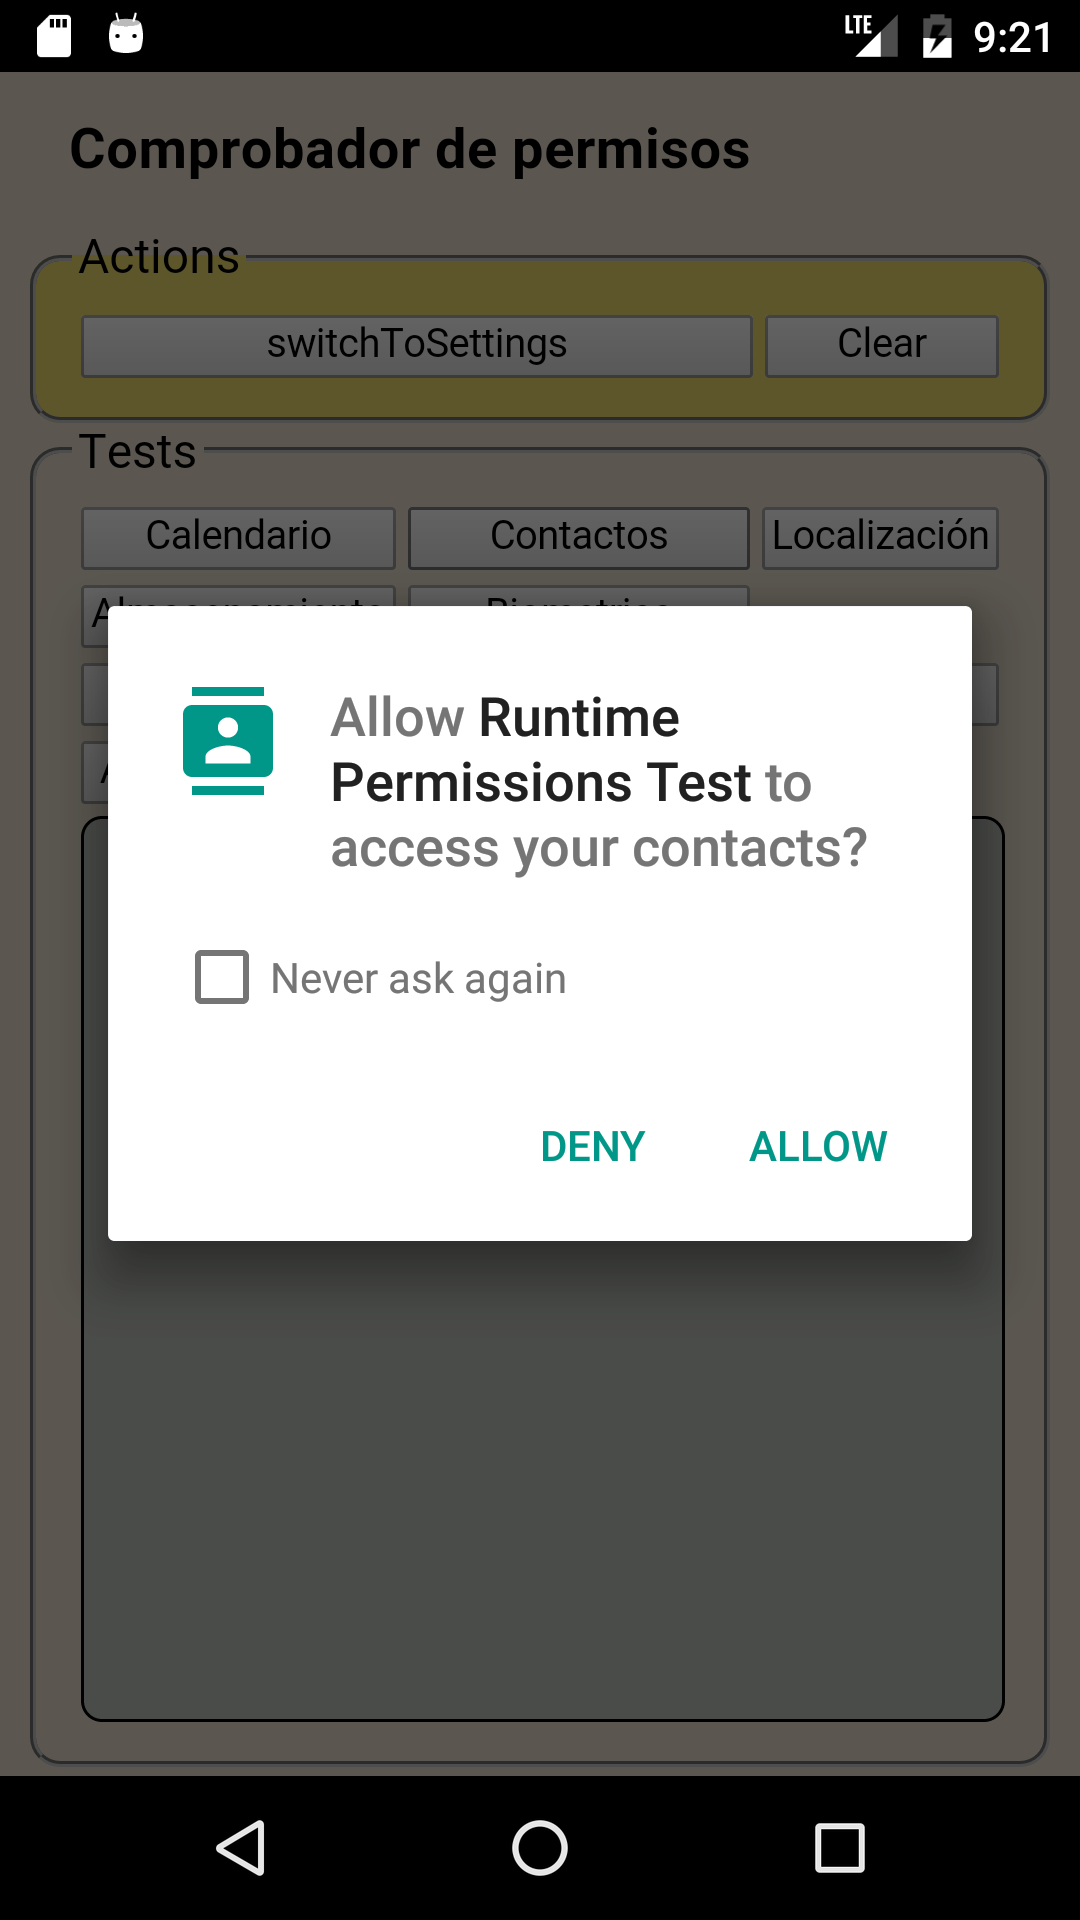
\includegraphics[width=\linewidth]{allow_contact}
    \end{subfigure}
    \begin{subfigure}{0.23\linewidth}
        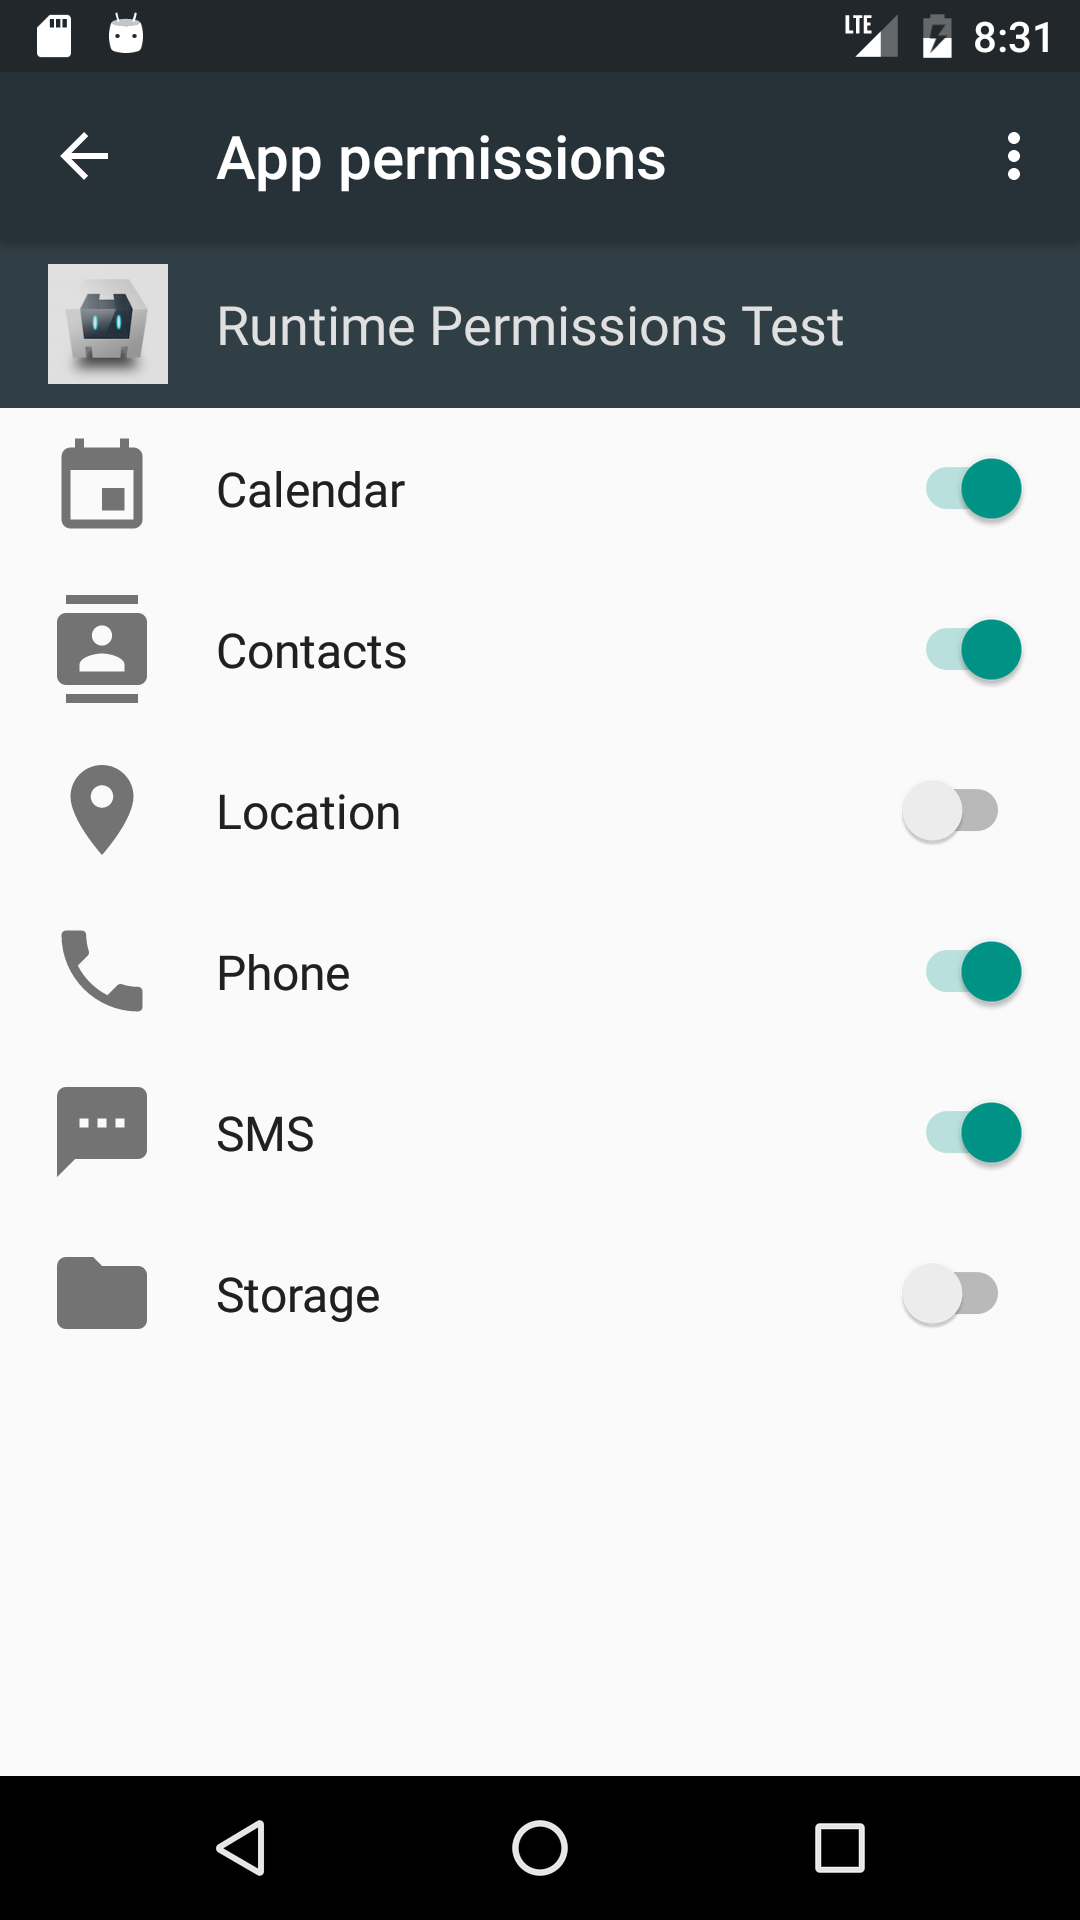
\includegraphics[width=\linewidth]{app-permissions}
	\end{subfigure}\pause
	\begin{subfigure}{.23\linewidth}
    	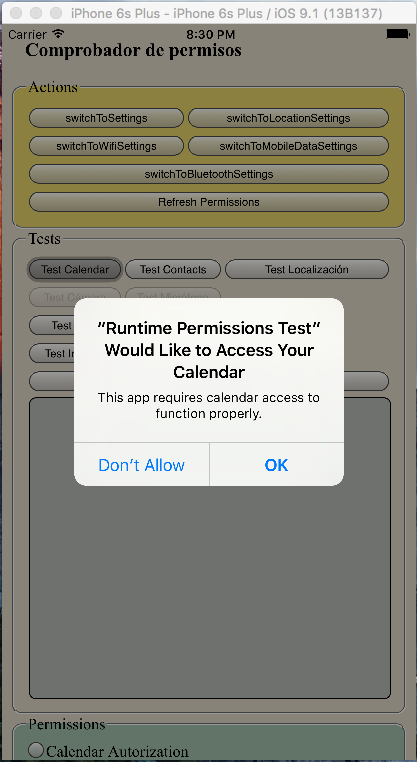
\includegraphics[width=\linewidth]{calendar_request_ios}
    \end{subfigure}
    \begin{subfigure}{.23\linewidth}
    	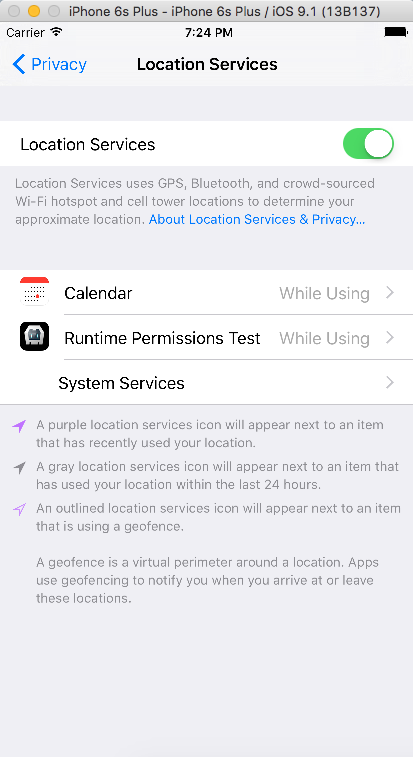
\includegraphics[width=\linewidth]{apps-allow-location}
	\end{subfigure}
\end{figure}
\end{frame}
\begin{frame}
 \frametitle{Análisis Comparativo}
Al comparar la gestión de permisos de ambas plataformas, encontramos varias similitudes:\pause
 \begin{itemize}[<+->]
  \item A una aplicación se le otorga permisos básicos al momento de instalación, sin posibilidad de revocarlos.
  \item Si una aplicación necesita un permiso no básico, debe requerirlo. El usuario puede otorgarlo o revocarlo.
  \item Desde la configuración de privacidad, el usuario puede revocar u otorgar permisos a las aplicaciones.
 \end{itemize}
\end{frame}
\begin{frame}
 \frametitle{Análisis Comparativo}
Respecto a cómo se definen los permisos, se observan diferencias de concepto:\\ \pause
 \begin{itemize}[<+->]
  \item En Android están orientados según el riesgo implícito al otorgarlos.
  \item En iOS los permisos están orientados a los componentes.
 \end{itemize} \pause
 
Sin embargo, se pueden comparar según los componentes que son afectados por un permiso, \pause resultando la siguiente Tabla:
  \begin{table}[H]
    \centering
    \begin{tiny}
	\begin{tabular}{c c c}
		\hline
		\multicolumn{3}{c}{\textbf{Permisos}} \\
		\emph{Ambas plataformas} 	& \emph{Solo en Android}	& \emph{Solo en iOS} \\ \hline    \hline
		Calendario	& -		& -	\\						
		Contactos	& -				& - \\						
		Cámara		& -				& -	\\						
		Localización& -				& -	\\						
		-			& -				& Compartir por Bluetooth\\ 
		Micrófono   & -				& - \\						
		-			& Teléfono		& -	\\						
		Sensores    & -    			& - \\						
		-			& SMS			& - \\						
		-			& Almacenamiento& - \\						
		-			& -				& \emph{Homekit} \\			
		-			& -				& Redes Sociales \\        	
		-			& -				& Diagnóstico \\        			
		-			& -				& Publicidad \\    			\hline
	\end{tabular}
	\end{tiny}
   \end{table}
\end{frame}
\begin{frame}
 \frametitle{Análisis Comparativo}
Respecto del alcance del sistema de permisos, se observó una falta de granularidad de los permisos que se pueden modificar \emph{en tiempo de ejecución}:\pause
  \begin{itemize}[<+->]
   \item En Android, un permiso es a nivel de grupo. Por lo tanto, el usuario otorga o deniega para todo el grupo.
   \item La misma situación ocurre en iOS: se otorga un permiso de acceso a todas las funcionalidades de un determinado componente.
  \end{itemize}
\pause Como consecuencia de ello, el usuario está delegando a una aplicación demasiados permisos y no tiene expresividad para decir qué funcionalidades autoriza.
\end{frame}
\begin{frame}
 \frametitle{Análisis Comparativo}
Otra cosa a destacar es la cobertura del sistema de permisos. \pause Las dos plataformas dejan funcionalidades principales del dispositivo sin permisos modificables \emph{en tiempo de ejecución}:\pause
  \begin{itemize}[<+->]
   \item En Android se destacan: Acceso a Internet, Compartir vía Bluetooth e Información del Dispositivo.
   \item En iOS se destacan: Acceso a Internet y SMS. Tampoco tiene la suficiente granularidad para administrar el acceso a los datos de las llamadas telefónicas.
  \end{itemize}
\end{frame}
\begin{frame}
 \frametitle{Análisis Comparativo}
Para finalizar analizamos cómo se muestran al usuario los permisos adquiridos por una aplicación:\pause
\begin{figure}
	\centering
	\begin{subfigure}{.25\linewidth}
		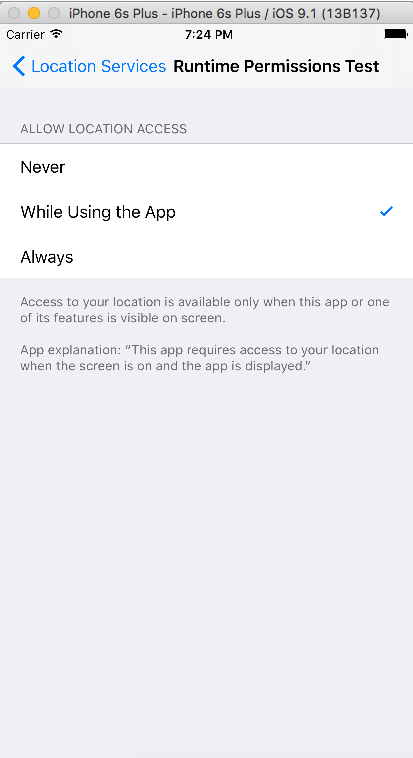
\includegraphics[width=\linewidth]{permission-classes.png}
		\caption{Permisos requeridos por una aplicación.}
		\label{fig:ch05:ios_all_permissions}
	\end{subfigure}\pause
	\begin{subfigure}{.25\linewidth}
		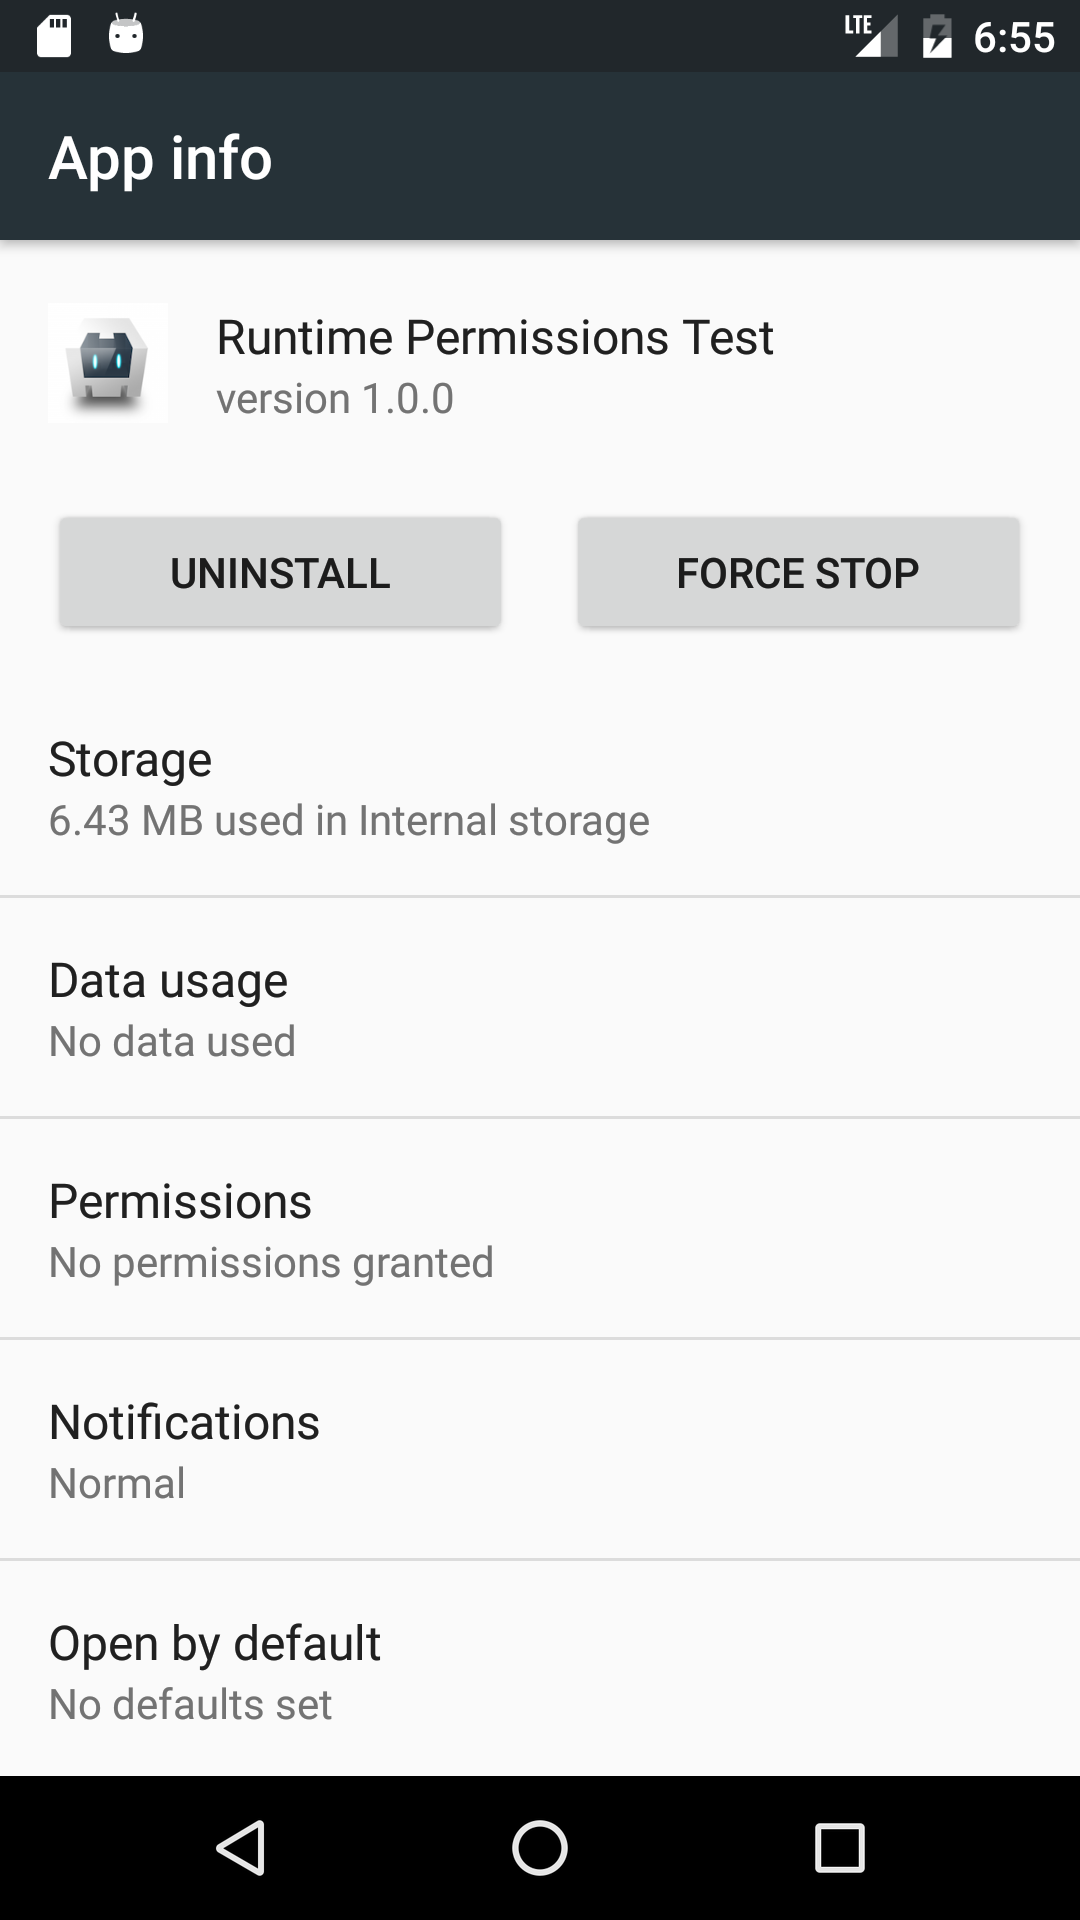
\includegraphics[width=\linewidth]{no_permissions_granted}
		\caption{La aplicación no tiene ningún permiso.}
		\label{fig:ch05:without_permissions}
	\end{subfigure}\pause
	\begin{subfigure}{.25\linewidth}
		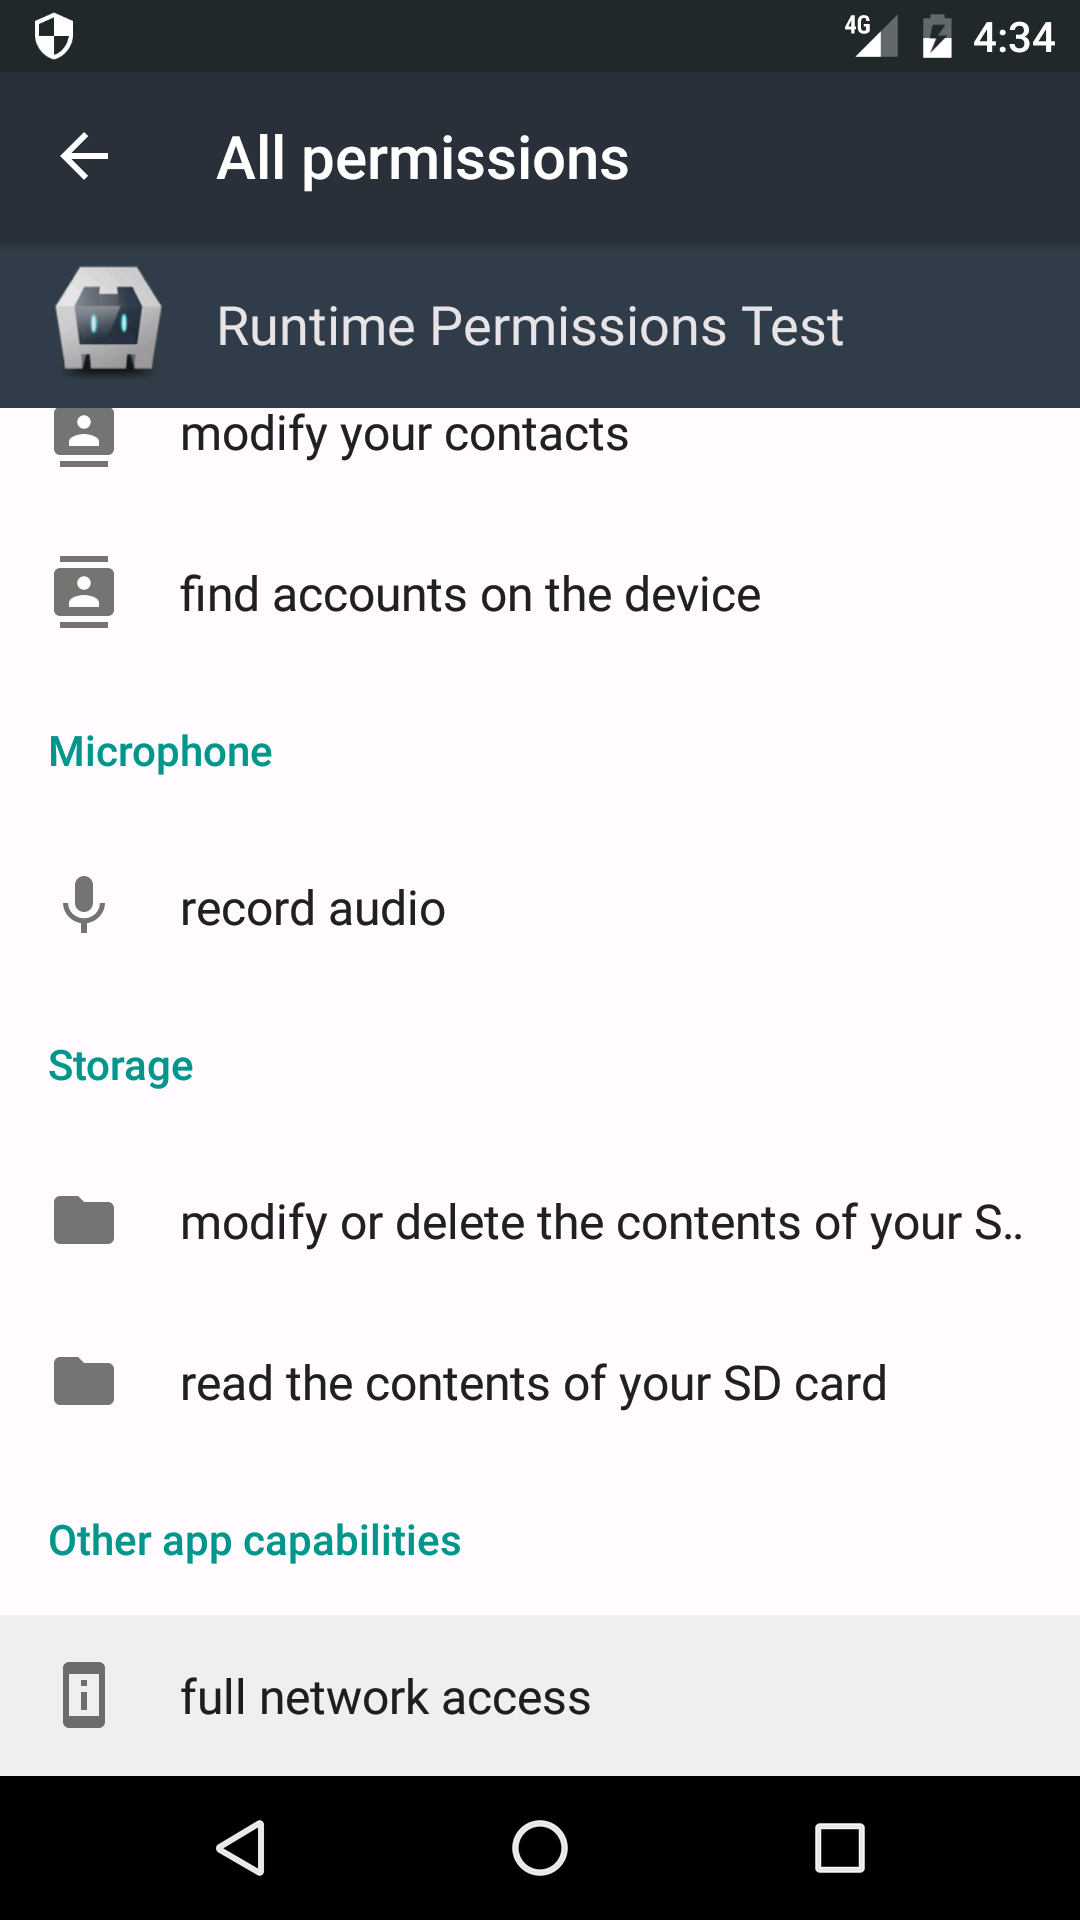
\includegraphics[width=\linewidth]{always_have_internet}
		\caption{Sin embargo, tiene todos los permisos \emph{normales}.}
		\label{fig:ch05:always_have_internet}
	\end{subfigure}
\end{figure}
\end{frame}